\documentclass[12pt,a4paper]{article}
\usepackage[utf8]{inputenc}
\usepackage[T1]{fontenc}
\usepackage{geometry}
\usepackage{tikz}
\usetikzlibrary{er,positioning,shapes.geometric,arrows.meta,shadows,fit,decorations.pathmorphing}
\usepackage{hyperref}
\usepackage{fancyhdr}
\usepackage{xcolor}
\usepackage{titlesec}
\usepackage{enumitem}
\usepackage{booktabs}
\usepackage{array}
\usepackage{tabularx}

\geometry{margin=1.5cm}
\pagestyle{fancy}
\fancyhf{}
\fancyhead[L]{GovEase - Entity-Relationship Diagram}
\fancyhead[R]{Team BitByBit}
\fancyfoot[C]{\thepage}

% Colors
\definecolor{primaryblue}{RGB}{59,130,246}
\definecolor{darkgray}{RGB}{75,85,99}
\definecolor{entitycolor}{RGB}{99,179,237}
\definecolor{attributecolor}{RGB}{255,235,59}
\definecolor{relationcolor}{RGB}{129,199,132}
\definecolor{primarykeycolor}{RGB}{244,67,54}

% Title formatting
\titleformat{\section}{\Large\bfseries\color{primaryblue}}{}{0em}{}
\titleformat{\subsection}{\large\bfseries\color{darkgray}}{}{0em}{}

\title{\textbf{\color{primaryblue}GovEase Government Services Management System\\Entity-Relationship Diagram}}
\author{\textbf{Team BitByBit - Tech-Triathlon 2025}}
\date{\today}

\begin{document}

\maketitle

\tableofcontents
\newpage

\section{Introduction}

This document presents the comprehensive Entity-Relationship Diagram (ERD) for the GovEase Government Services Management System. The ERD illustrates the data model, entity relationships, and database structure that supports the platform's core functionalities including appointment booking, document management, notifications, and analytics.

\subsection{Database Design Principles}
\begin{itemize}[leftmargin=*]
    \item \textbf{Normalization}: Database is designed in 3NF to eliminate redundancy
    \item \textbf{Scalability}: Structure supports horizontal scaling for government-level usage
    \item \textbf{Security}: Role-based access control and audit trails built into the schema
    \item \textbf{Performance}: Optimized for Firebase Firestore NoSQL operations
\end{itemize}

\section{Entity-Relationship Diagram}

\begin{figure}[h!]
\centering
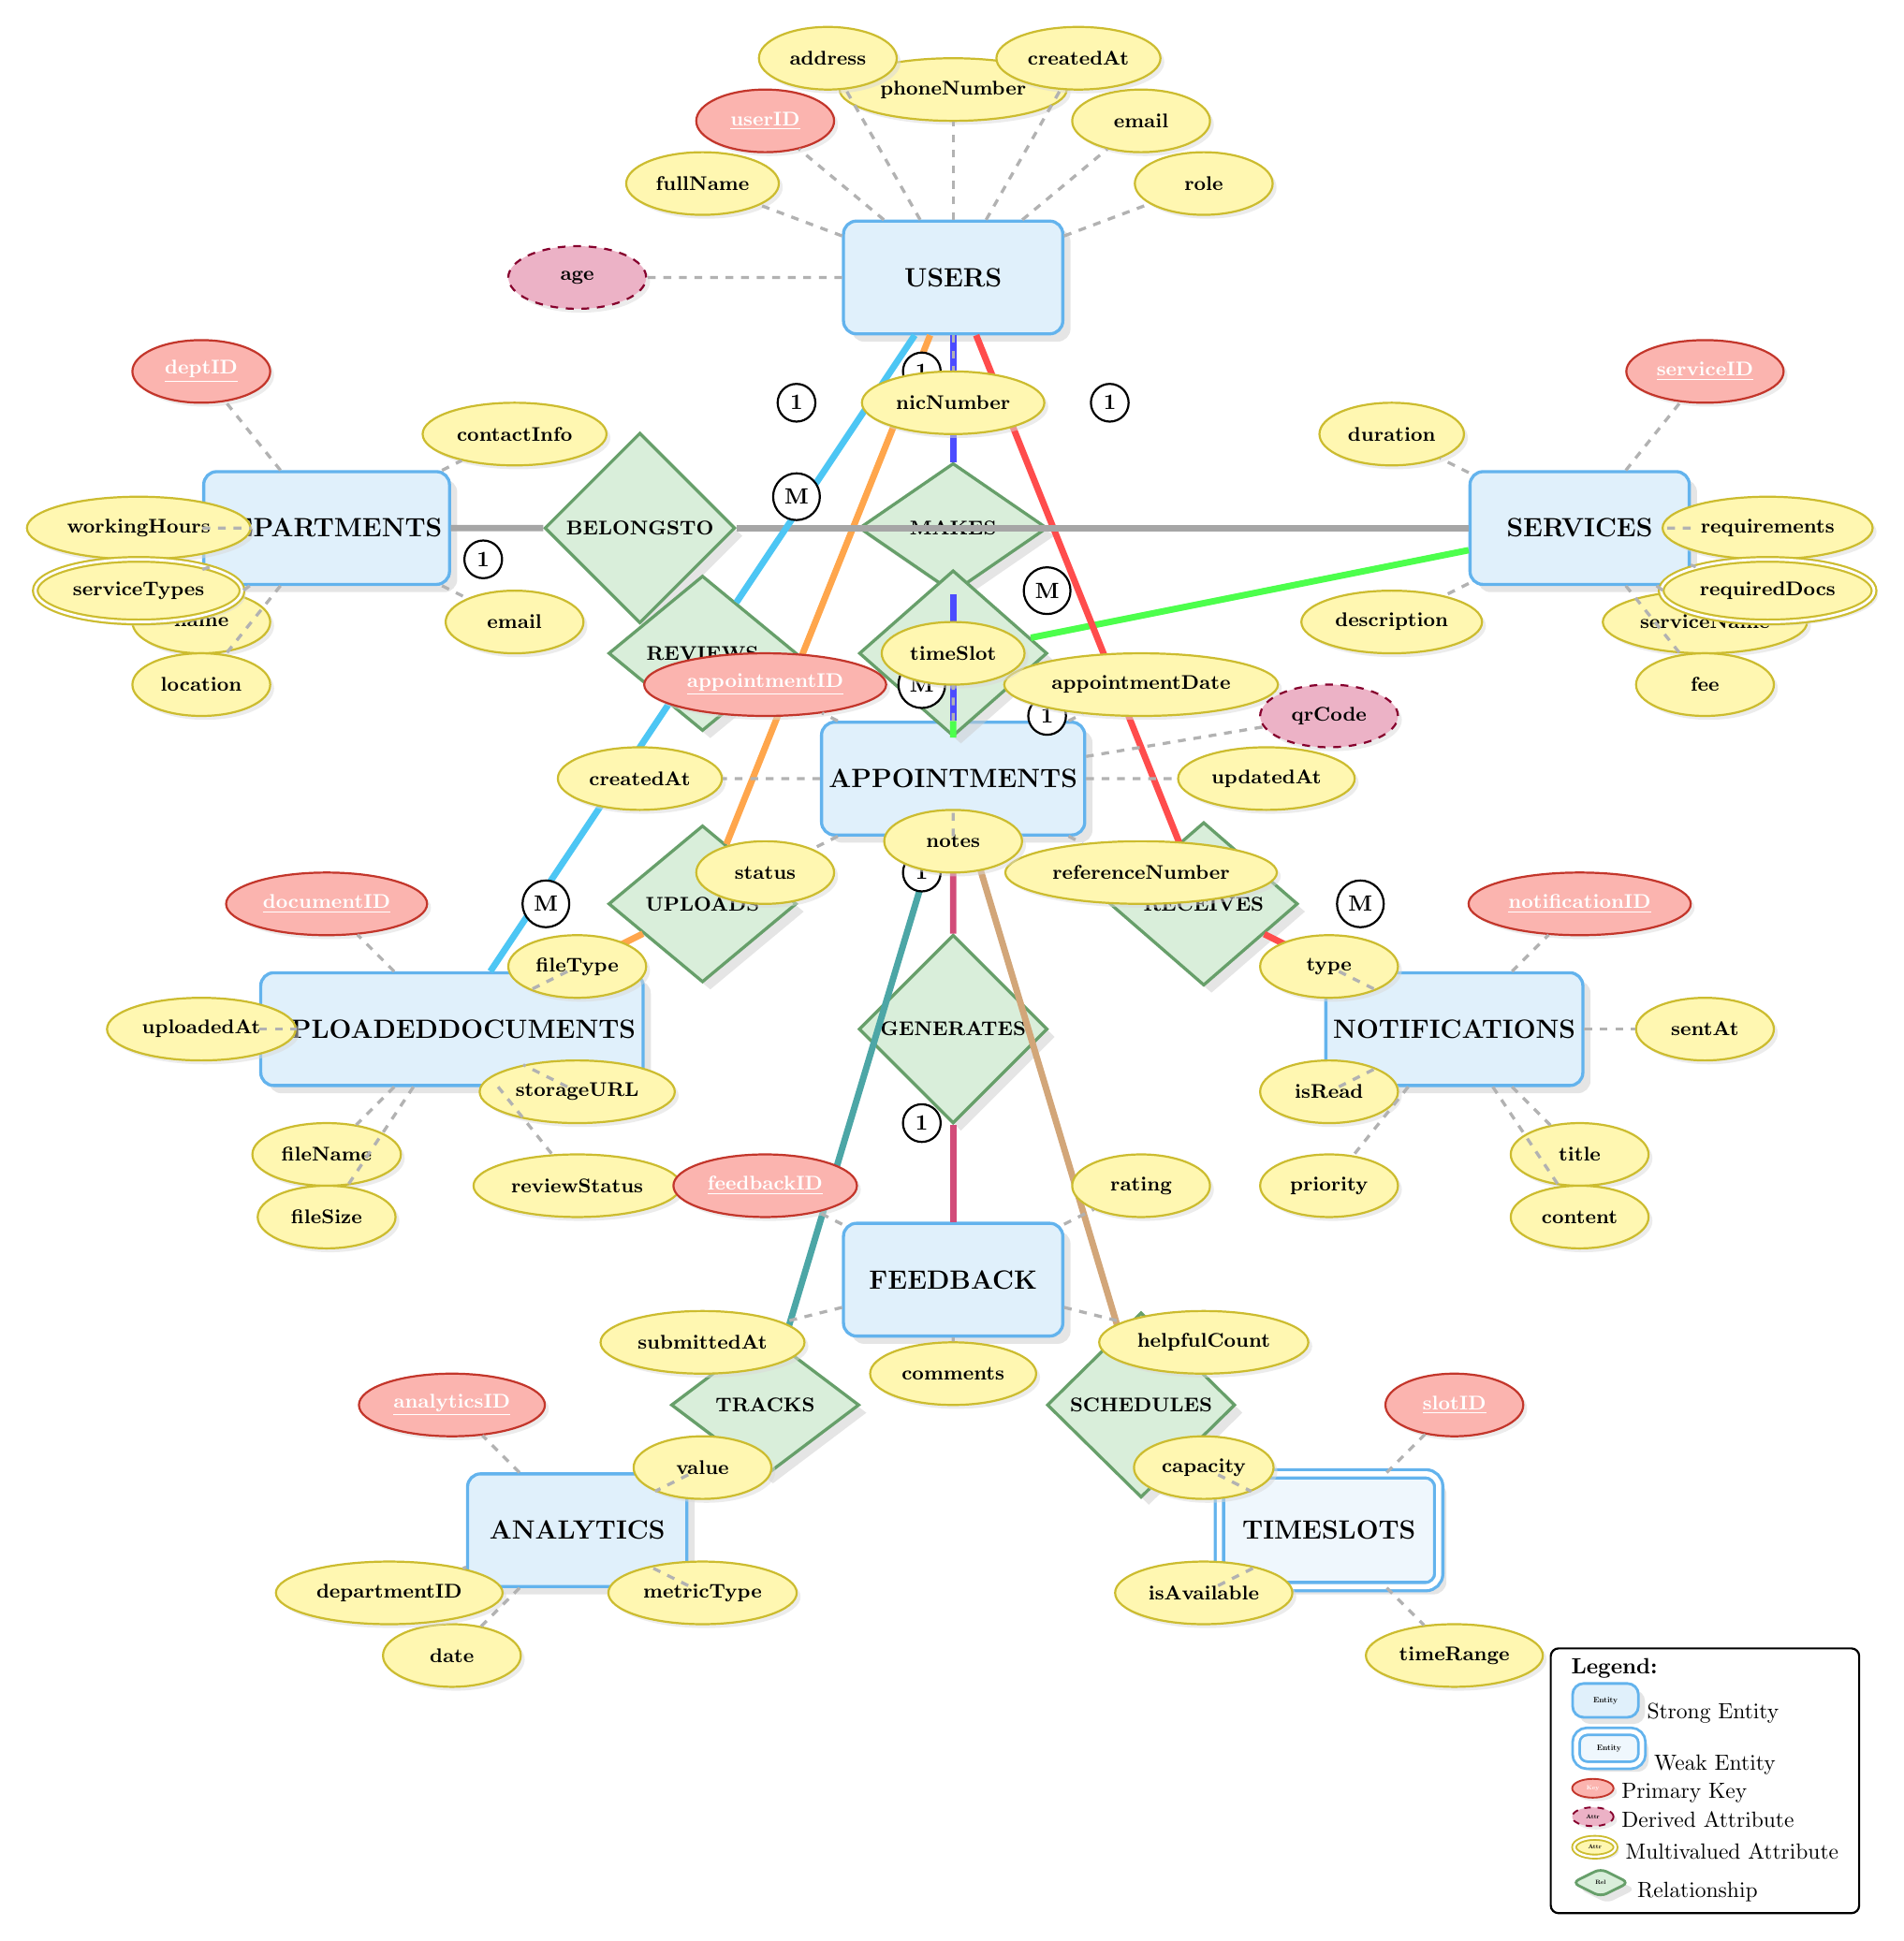
\begin{tikzpicture}[node distance=1.8cm, auto, scale=0.85, transform shape]

% Enhanced styles with modern design
\tikzstyle{entity} = [rectangle, draw=entitycolor, very thick, text centered, 
                     minimum height=1.8cm, minimum width=3.5cm, 
                     fill=entitycolor!20, rounded corners=5pt, font=\bfseries\large,
                     drop shadow={shadow xshift=3pt, shadow yshift=-3pt, fill=gray!40}]

\tikzstyle{weakentity} = [rectangle, draw=entitycolor, very thick, text centered, 
                         minimum height=1.8cm, minimum width=3.5cm, 
                         fill=entitycolor!10, rounded corners=5pt, font=\bfseries\large,
                         double, double distance=2pt,
                         drop shadow={shadow xshift=3pt, shadow yshift=-3pt, fill=gray!40}]
                     
\tikzstyle{attribute} = [ellipse, draw=attributecolor!80!black, thick, text centered, 
                        minimum height=1cm, minimum width=2.2cm, 
                        fill=attributecolor!40, font=\small\bfseries,
                        drop shadow={shadow xshift=1.5pt, shadow yshift=-1.5pt, fill=gray!30}]
                        
\tikzstyle{relationship} = [diamond, draw=relationcolor!80!black, very thick, text centered, 
                           minimum height=1.5cm, minimum width=3cm, 
                           fill=relationcolor!30, font=\bfseries\small,
                           drop shadow={shadow xshift=3pt, shadow yshift=-3pt, fill=gray!40}]
                           
\tikzstyle{primarykey} = [attribute, fill=primarykeycolor!40, draw=primarykeycolor!80!black, 
                         font=\small\bfseries, text=white]

\tikzstyle{derived} = [attribute, fill=purple!30, draw=purple!70!black, 
                      font=\small\bfseries, dashed]

\tikzstyle{multivalued} = [attribute, double, double distance=1pt]

% Core entities positioned strategically
\node [entity] (users) at (0,12) {USERS};
\node [entity] (departments) at (-10,8) {DEPARTMENTS};
\node [entity] (services) at (10,8) {SERVICES};
\node [entity] (appointments) at (0,4) {APPOINTMENTS};
\node [entity] (documents) at (-8,0) {UPLOADED\\DOCUMENTS};
\node [entity] (notifications) at (8,0) {NOTIFICATIONS};
\node [entity] (feedback) at (0,-4) {FEEDBACK};
\node [entity] (analytics) at (-6,-8) {ANALYTICS};
\node [weakentity] (slots) at (6,-8) {TIME\\SLOTS};

% Relationship diamonds
\node [relationship] (makes) at (0,8) {MAKES};
\node [relationship] (provides) at (0,6) {PROVIDES};
\node [relationship] (uploads) at (-4,2) {UPLOADS};
\node [relationship] (receives) at (4,2) {RECEIVES};
\node [relationship] (generates) at (0,0) {GENERATES};
\node [relationship] (tracks) at (-3,-6) {TRACKS};
\node [relationship] (schedules) at (3,-6) {SCHEDULES};
\node [relationship] (belongs_dept) at (-5,8) {BELONGS\\TO};
\node [relationship] (reviews) at (-4,6) {REVIEWS};

% Main relationship lines with enhanced styling
\draw [line width=2.5pt, blue!70] (users) -- (makes);
\draw [line width=2.5pt, blue!70] (makes) -- (appointments);
\draw [line width=2.5pt, green!70] (services) -- (provides);
\draw [line width=2.5pt, green!70] (provides) -- (appointments);
\draw [line width=2.5pt, orange!70] (users) -- (uploads);
\draw [line width=2.5pt, orange!70] (uploads) -- (documents);
\draw [line width=2.5pt, red!70] (users) -- (receives);
\draw [line width=2.5pt, red!70] (receives) -- (notifications);
\draw [line width=2.5pt, purple!70] (appointments) -- (generates);
\draw [line width=2.5pt, purple!70] (generates) -- (feedback);
\draw [line width=2.5pt, teal!70] (appointments) -- (tracks);
\draw [line width=2.5pt, teal!70] (tracks) -- (analytics);
\draw [line width=2.5pt, brown!70] (appointments) -- (schedules);
\draw [line width=2.5pt, brown!70] (schedules) -- (slots);
\draw [line width=2.5pt, gray!70] (departments) -- (belongs_dept);
\draw [line width=2.5pt, gray!70] (belongs_dept) -- (services);
\draw [line width=2.5pt, cyan!70] (users) -- (reviews);
\draw [line width=2.5pt, cyan!70] (reviews) -- (documents);

% Enhanced cardinality labels with better visibility
\node [font=\bfseries, fill=white, circle, inner sep=3pt, draw=black, thick] at (-0.5,10.5) {1};
\node [font=\bfseries, fill=white, circle, inner sep=3pt, draw=black, thick] at (-0.5,5.5) {M};
\node [font=\bfseries, fill=white, circle, inner sep=3pt, draw=black, thick] at (1.5,7) {M};
\node [font=\bfseries, fill=white, circle, inner sep=3pt, draw=black, thick] at (1.5,5) {1};
\node [font=\bfseries, fill=white, circle, inner sep=3pt, draw=black, thick] at (-2.5,10) {1};
\node [font=\bfseries, fill=white, circle, inner sep=3pt, draw=black, thick] at (-6.5,2) {M};
\node [font=\bfseries, fill=white, circle, inner sep=3pt, draw=black, thick] at (2.5,10) {1};
\node [font=\bfseries, fill=white, circle, inner sep=3pt, draw=black, thick] at (6.5,2) {M};
\node [font=\bfseries, fill=white, circle, inner sep=3pt, draw=black, thick] at (-0.5,2.5) {1};
\node [font=\bfseries, fill=white, circle, inner sep=3pt, draw=black, thick] at (-0.5,-1.5) {1};
\node [font=\bfseries, fill=white, circle, inner sep=3pt, draw=black, thick] at (-7.5,7.5) {1};
\node [font=\bfseries, fill=white, circle, inner sep=3pt, draw=black, thick] at (-2.5,8.5) {M};

% USERS attributes - comprehensive and well-organized
\node [primarykey] (user_id) at (-3,14.5) {\underline{userID}};
\node [attribute] (user_email) at (3,14.5) {email};
\node [attribute] (user_name) at (-4,13.5) {fullName};
\node [attribute] (user_role) at (4,13.5) {role};
\node [attribute] (user_phone) at (0,15) {phoneNumber};
\node [attribute] (user_nic) at (0,10) {nicNumber};
\node [attribute] (user_address) at (-2,15.5) {address};
\node [attribute] (user_created) at (2,15.5) {createdAt};
\node [derived] (user_age) at (-6,12) {age};

% DEPARTMENTS attributes
\node [primarykey] (dept_id) at (-12,10.5) {\underline{deptID}};
\node [attribute] (dept_name) at (-12,6.5) {name};
\node [attribute] (dept_location) at (-12,5.5) {location};
\node [attribute] (dept_contact) at (-7,9.5) {contactInfo};
\node [attribute] (dept_email) at (-7,6.5) {email};
\node [attribute] (dept_hours) at (-13,8) {workingHours};
\node [multivalued] (dept_services) at (-13,7) {serviceTypes};

% SERVICES attributes
\node [primarykey] (service_id) at (12,10.5) {\underline{serviceID}};
\node [attribute] (service_name) at (12,6.5) {serviceName};
\node [attribute] (service_fee) at (12,5.5) {fee};
\node [attribute] (service_duration) at (7,9.5) {duration};
\node [attribute] (service_description) at (7,6.5) {description};
\node [attribute] (service_requirements) at (13,8) {requirements};
\node [multivalued] (service_docs) at (13,7) {requiredDocs};

% APPOINTMENTS attributes - enhanced
\node [primarykey] (apt_id) at (-3,5.5) {\underline{appointmentID}};
\node [attribute] (apt_date) at (3,5.5) {appointmentDate};
\node [attribute] (apt_status) at (-3,2.5) {status};
\node [attribute] (apt_ref) at (3,2.5) {referenceNumber};
\node [attribute] (apt_slot) at (0,6) {timeSlot};
\node [attribute] (apt_created) at (-5,4) {createdAt};
\node [attribute] (apt_updated) at (5,4) {updatedAt};
\node [attribute] (apt_notes) at (0,3) {notes};
\node [derived] (apt_qr) at (6,5) {qrCode};

% DOCUMENTS attributes
\node [primarykey] (doc_id) at (-10,2) {\underline{documentID}};
\node [attribute] (doc_name) at (-10,-2) {fileName};
\node [attribute] (doc_type) at (-6,1) {fileType};
\node [attribute] (doc_url) at (-6,-1) {storageURL};
\node [attribute] (doc_size) at (-10,-3) {fileSize};
\node [attribute] (doc_status) at (-6,-2.5) {reviewStatus};
\node [attribute] (doc_uploaded) at (-12,0) {uploadedAt};

% NOTIFICATIONS attributes
\node [primarykey] (notif_id) at (10,2) {\underline{notificationID}};
\node [attribute] (notif_title) at (10,-2) {title};
\node [attribute] (notif_type) at (6,1) {type};
\node [attribute] (notif_read) at (6,-1) {isRead};
\node [attribute] (notif_content) at (10,-3) {content};
\node [attribute] (notif_sent) at (12,0) {sentAt};
\node [attribute] (notif_priority) at (6,-2.5) {priority};

% FEEDBACK attributes
\node [primarykey] (feed_id) at (-3,-2.5) {\underline{feedbackID}};
\node [attribute] (feed_rating) at (3,-2.5) {rating};
\node [attribute] (feed_comment) at (0,-5.5) {comments};
\node [attribute] (feed_date) at (-4,-5) {submittedAt};
\node [attribute] (feed_helpful) at (4,-5) {helpfulCount};

% ANALYTICS attributes
\node [primarykey] (analytics_id) at (-8,-6) {\underline{analyticsID}};
\node [attribute] (analytics_date) at (-8,-10) {date};
\node [attribute] (analytics_metric) at (-4,-9) {metricType};
\node [attribute] (analytics_value) at (-4,-7) {value};
\node [attribute] (analytics_dept) at (-9,-9) {departmentID};

% TIME SLOTS attributes
\node [primarykey] (slot_id) at (8,-6) {\underline{slotID}};
\node [attribute] (slot_time) at (8,-10) {timeRange};
\node [attribute] (slot_available) at (4,-9) {isAvailable};
\node [attribute] (slot_capacity) at (4,-7) {capacity};

% Connect attributes to entities with elegant lines
\foreach \attr in {user_id, user_email, user_name, user_role, user_phone, user_nic, user_address, user_created, user_age} {
    \draw [dashed, gray!60, line width=1.2pt] (users) -- (\attr);
}

\foreach \attr in {dept_id, dept_name, dept_location, dept_contact, dept_email, dept_hours, dept_services} {
    \draw [dashed, gray!60, line width=1.2pt] (departments) -- (\attr);
}

\foreach \attr in {service_id, service_name, service_fee, service_duration, service_description, service_requirements, service_docs} {
    \draw [dashed, gray!60, line width=1.2pt] (services) -- (\attr);
}

\foreach \attr in {apt_id, apt_date, apt_status, apt_ref, apt_slot, apt_created, apt_updated, apt_notes, apt_qr} {
    \draw [dashed, gray!60, line width=1.2pt] (appointments) -- (\attr);
}

\foreach \attr in {doc_id, doc_name, doc_type, doc_url, doc_size, doc_status, doc_uploaded} {
    \draw [dashed, gray!60, line width=1.2pt] (documents) -- (\attr);
}

\foreach \attr in {notif_id, notif_title, notif_type, notif_read, notif_content, notif_sent, notif_priority} {
    \draw [dashed, gray!60, line width=1.2pt] (notifications) -- (\attr);
}

\foreach \attr in {feed_id, feed_rating, feed_comment, feed_date, feed_helpful} {
    \draw [dashed, gray!60, line width=1.2pt] (feedback) -- (\attr);
}

\foreach \attr in {analytics_id, analytics_date, analytics_metric, analytics_value, analytics_dept} {
    \draw [dashed, gray!60, line width=1.2pt] (analytics) -- (\attr);
}

\foreach \attr in {slot_id, slot_time, slot_available, slot_capacity} {
    \draw [dashed, gray!60, line width=1.2pt] (slots) -- (\attr);
}

% Add legend
\node [draw=black, thick, fill=white, rounded corners=3pt] at (12,-12) {
    \begin{tabular}{l}
        \textbf{Legend:} \\
        \tikz\node[entity,scale=0.3]{Entity}; Strong Entity \\
        \tikz\node[weakentity,scale=0.3]{Entity}; Weak Entity \\
        \tikz\node[primarykey,scale=0.3]{Key}; Primary Key \\
        \tikz\node[derived,scale=0.3]{Attr}; Derived Attribute \\
        \tikz\node[multivalued,scale=0.3]{Attr}; Multivalued Attribute \\
        \tikz\node[relationship,scale=0.3]{Rel}; Relationship
    \end{tabular}
};

\end{tikzpicture}
\caption{Comprehensive Entity-Relationship Diagram for GovEase Database Schema}
\label{fig:complete_er_diagram}
\end{figure}

\newpage

\section{Entity Descriptions}

\subsection{Core Entities}

\subsubsection{USERS}
Central entity representing all system users including citizens, government officers, and administrators.
\begin{itemize}[leftmargin=*]
    \item \textbf{Primary Key}: userID (UUID)
    \item \textbf{Attributes}: email, fullName, role (citizen/officer/admin), phoneNumber, nicNumber, address, createdAt
    \item \textbf{Derived Attribute}: age (calculated from NIC number)
    \item \textbf{Role Values}: 'citizen', 'officer', 'admin'
\end{itemize}

\subsubsection{DEPARTMENTS}
Government departments that provide various services to citizens.
\begin{itemize}[leftmargin=*]
    \item \textbf{Primary Key}: deptID (UUID)
    \item \textbf{Attributes}: name, location, contactInfo, email, workingHours
    \item \textbf{Multivalued}: serviceTypes (array of service categories)
    \item \textbf{Examples}: Department of Motor Traffic, Immigration \& Emigration, Registrar General
\end{itemize}

\subsubsection{SERVICES}
Specific services offered by government departments.
\begin{itemize}[leftmargin=*]
    \item \textbf{Primary Key}: serviceID (UUID)
    \item \textbf{Attributes}: serviceName, fee, duration, description, requirements
    \item \textbf{Multivalued}: requiredDocs (array of required document types)
    \item \textbf{Examples}: Driving License Application, Passport Renewal, Birth Certificate
\end{itemize}

\subsubsection{APPOINTMENTS}
Scheduled appointments between citizens and government services.
\begin{itemize}[leftmargin=*]
    \item \textbf{Primary Key}: appointmentID (UUID)
    \item \textbf{Attributes}: appointmentDate, status, referenceNumber, timeSlot, createdAt, updatedAt, notes
    \item \textbf{Derived}: qrCode (generated from appointmentID)
    \item \textbf{Status Values}: 'pending', 'confirmed', 'completed', 'cancelled', 'no-show'
\end{itemize}

\subsection{Supporting Entities}

\subsubsection{UPLOADED DOCUMENTS}
Files and documents uploaded by users for their appointments.
\begin{itemize}[leftmargin=*]
    \item \textbf{Primary Key}: documentID (UUID)
    \item \textbf{Attributes}: fileName, fileType, storageURL, fileSize, reviewStatus, uploadedAt
    \item \textbf{Review Status}: 'pending', 'approved', 'rejected', 'resubmission_required'
\end{itemize}

\subsubsection{NOTIFICATIONS}
System-generated notifications sent to users.
\begin{itemize}[leftmargin=*]
    \item \textbf{Primary Key}: notificationID (UUID)
    \item \textbf{Attributes}: title, type, content, isRead, sentAt, priority
    \item \textbf{Types}: 'appointment_reminder', 'status_update', 'document_review', 'system_alert'
\end{itemize}

\subsubsection{FEEDBACK}
User feedback and ratings for completed appointments.
\begin{itemize}[leftmargin=*]
    \item \textbf{Primary Key}: feedbackID (UUID)
    \item \textbf{Attributes}: rating (1-5 stars), comments, submittedAt, helpfulCount
    \item \textbf{Rating Scale}: 1 (Poor) to 5 (Excellent)
\end{itemize}

\subsubsection{ANALYTICS}
System analytics and performance metrics.
\begin{itemize}[leftmargin=*]
    \item \textbf{Primary Key}: analyticsID (UUID)
    \item \textbf{Attributes}: date, metricType, value, departmentID
    \item \textbf{Metric Types}: 'appointments_count', 'completion_rate', 'satisfaction_score', 'no_show_rate'
\end{itemize}

\subsubsection{TIME SLOTS (Weak Entity)}
Available time slots for appointments, dependent on services.
\begin{itemize}[leftmargin=*]
    \item \textbf{Primary Key}: slotID (composite with serviceID)
    \item \textbf{Attributes}: timeRange, isAvailable, capacity
    \item \textbf{Dependency}: Existence depends on SERVICES entity
\end{itemize}

\newpage

\section{Relationship Analysis}

\subsection{Primary Relationships}

\begin{table}[h!]
\centering
\begin{tabularx}{\textwidth}{|X|X|X|X|}
\hline
\textbf{Relationship} & \textbf{Entities} & \textbf{Cardinality} & \textbf{Description} \\
\hline
MAKES & USERS ↔ APPOINTMENTS & 1:M & Each user can make multiple appointments \\
\hline
PROVIDES & SERVICES ↔ APPOINTMENTS & 1:M & Each service can have multiple appointments \\
\hline
UPLOADS & USERS ↔ DOCUMENTS & 1:M & Each user can upload multiple documents \\
\hline
RECEIVES & USERS ↔ NOTIFICATIONS & 1:M & Each user can receive multiple notifications \\
\hline
GENERATES & APPOINTMENTS ↔ FEEDBACK & 1:1 & Each appointment generates one feedback \\
\hline
BELONGS TO & DEPARTMENTS ↔ SERVICES & 1:M & Each department offers multiple services \\
\hline
TRACKS & APPOINTMENTS ↔ ANALYTICS & M:1 & Multiple appointments contribute to analytics \\
\hline
SCHEDULES & APPOINTMENTS ↔ TIME SLOTS & M:1 & Multiple appointments use time slots \\
\hline
REVIEWS & USERS ↔ DOCUMENTS & 1:M & Officers review multiple documents \\
\hline
\end{tabularx}
\caption{Complete Relationship Matrix}
\label{tab:relationships}
\end{table}

\subsection{Relationship Constraints}

\subsubsection{Business Rules}
\begin{enumerate}[leftmargin=*]
    \item A citizen cannot book multiple appointments for the same service on the same day
    \item Officers can only review documents for services within their department
    \item Feedback can only be submitted after appointment completion
    \item Time slots have maximum capacity constraints
    \item Documents must be uploaded before appointment confirmation
    \item Notifications are automatically generated for appointment status changes
\end{enumerate}

\subsubsection{Referential Integrity}
\begin{itemize}[leftmargin=*]
    \item All foreign keys maintain referential integrity
    \item Cascade delete operations for dependent entities
    \item Soft delete implementation for audit trail preservation
    \item Composite keys for weak entities ensure proper dependency
\end{itemize}

\section{Database Implementation Notes}

\subsection{Firebase Firestore Mapping}

\subsubsection{Collection Structure}
\begin{verbatim}
/users/{userID}
/departments/{deptID}
/services/{serviceID}
/appointments/{appointmentID}
/uploaded_documents/{documentID}
/notifications/{notificationID}
/feedback/{feedbackID}
/analytics/{analyticsID}
/time_slots/{slotID}
\end{verbatim}

\subsubsection{Security Rules}
\begin{itemize}[leftmargin=*]
    \item Role-based access control implemented through custom claims
    \item Users can only access their own data (except officers/admins)
    \item Officers have read/write access to their department's data
    \item Admins have full system access with audit logging
\end{itemize}

\subsection{Performance Optimizations}

\subsubsection{Indexing Strategy}
\begin{itemize}[leftmargin=*]
    \item Composite indexes on frequently queried field combinations
    \item Single-field indexes on all foreign keys
    \item Text search indexes for service and department names
    \item Time-based indexes for appointment scheduling queries
\end{itemize}

\subsubsection{Query Optimization}
\begin{itemize}[leftmargin=*]
    \item Denormalization of frequently accessed data
    \item Pagination for large result sets
    \item Real-time listeners for critical updates
    \item Cached computed values for analytics
\end{itemize}

\section{Data Validation Rules}

\subsection{Field Constraints}
\begin{table}[h!]
\centering
\begin{tabularx}{\textwidth}{|X|X|X|}
\hline
\textbf{Field} & \textbf{Constraint} & \textbf{Validation Rule} \\
\hline
email & Unique, Required & Valid email format, domain whitelist \\
\hline
nicNumber & Unique, Required & Sri Lankan NIC format validation \\
\hline
phoneNumber & Required & Sri Lankan mobile number format \\
\hline
appointmentDate & Required & Future date, business hours only \\
\hline
rating & Required & Integer between 1-5 \\
\hline
fileSize & Required & Maximum 10MB per document \\
\hline
timeSlot & Required & Valid time format, availability check \\
\hline
\end{tabularx}
\caption{Data Validation Constraints}
\label{tab:validation}
\end{table}

\subsection{Business Logic Validation}
\begin{itemize}[leftmargin=*]
    \item Appointment time conflicts prevention
    \item Service prerequisite validation
    \item Document type verification against service requirements
    \item User role permissions enforcement
    \item Audit trail maintenance for all data modifications
\end{itemize}

\section{Conclusion}

This comprehensive ER diagram represents a robust, scalable database design for the GovEase platform. The schema supports all current functionalities while providing flexibility for future enhancements. The design emphasizes data integrity, security, and performance optimization suitable for government-scale operations.

The normalized structure ensures data consistency while strategic denormalization optimizes query performance. Security measures and audit trails meet government data protection requirements, making this design production-ready for national deployment.

\end{document}